\documentclass[11pt]{article}

\usepackage{times}
\usepackage{epsf}
\usepackage{epsfig}
\usepackage{amsmath, alltt, amssymb, xspace}
\usepackage{wrapfig}
\usepackage{fancyhdr}
\usepackage{url}
\usepackage{verbatim}
\usepackage{fancyvrb}
\usepackage{float}

\usepackage{subfigure}
\usepackage{cite}
\usepackage{hyperref}
\hypersetup{%
    pdfborder = {0 0 0}
}
\topmargin      -0.50in  % distance to headers
\oddsidemargin  0.0in
\evensidemargin 0.0in
\textwidth      6.5in
\textheight     8.9in


%\centerfigcaptionstrue

%\def\baselinestretch{0.95}


\newcommand\discuss[1]{\{\textbf{Discuss:} \textit{#1}\}}
%\newcommand\todo[1]{\vspace{0.1in}\{\textbf{Todo:} \textit{#1}\}\vspace{0.1in}}
\newtheorem{problem}{Problem}[section]
%\newtheorem{theorem}{Theorem}
%\newtheorem{fact}{Fact}
\newtheorem{define}{Definition}[section]
%\newtheorem{analysis}{Analysis}
\newcommand\vspacenoindent{\vspace{0.1in} \noindent}

%\newenvironment{proof}{\noindent {\bf Proof}.}{\hspace*{\fill}~\mbox{\rule[0pt]{1.3ex}{1.3ex}}}
%\newcommand\todo[1]{\vspace{0.1in}\{\textbf{Todo:} \textit{#1}\}\vspace{0.1in}}

%\newcommand\reducespace{\vspace{-0.1in}}
% reduce the space between lines
%\def\baselinestretch{0.95}

\newcommand{\fixmefn}[1]{ \footnote{\sf\ \ \fbox{FIXME} #1} }
\newcommand{\todo}[1]{
\vspace{0.1in}
\fbox{\parbox{6in}{TODO: #1}}
\vspace{0.1in}
}

\newcommand{\mybox}[1]{
\vspace{0.2in}
\noindent
\fbox{\parbox{6.5in}{#1}}
\vspace{0.1in}
}


\newcounter{question}
\setcounter{question}{1}

\newcommand{\myquestion} {{\vspace{0.1in} \noindent \bf Question \arabic{question}:} \addtocounter{question}{1} \,}

\newcommand{\myproblem} {{\noindent \bf Problem \arabic{question}:} \addtocounter{question}{1} \,}



\newcommand{\copyrightnotice}[1]{
\vspace{0.1in}
\fbox{\parbox{6in}{
			This lab was developed by Sparta Global for Cybersecurity courses.
			It was built based on the original lab that was developed for the Labtainer framework by the Naval Postgraduate School, Center for Cybersecurity and Cyber Operations under National Science Foundation Award No. 1438893.
      This work is in the public domain, and cannot be copyrighted.
			}}
\vspace{0.1in}
}


\newcommand{\idea}[1]{
\vspace{0.1in}
{\sf IDEA:\ \ \fbox{\parbox{5in}{#1}}}
\vspace{0.1in}
}

\newcommand{\questionblock}[1]{
\vspace{0.1in}
\fbox{\parbox{6in}{#1}}
\vspace{0.1in}
}


\newcommand{\argmax}[1]{
\begin{minipage}[t]{1.25cm}\parskip-1ex\begin{center}
argmax
#1
\end{center}\end{minipage}
\;
}

\newcommand{\bm}{\boldmath}
\newcommand  {\bx}    {\mbox{\boldmath $x$}}
\newcommand  {\by}    {\mbox{\boldmath $y$}}
\newcommand  {\br}    {\mbox{\boldmath $r$}}


\newcommand{\tstamp}{\today}
%\rfoot[\fancyplain{\tstamp} {\tstamp}]  {\fancyplain{}{}}

\pagestyle{fancy}
\lhead{\bfseries Labtainers}
\chead{}
\rhead{\small \thepage}
\lfoot{\small{\textit{Dr. Osama Abu Oun - Cybersecurity Courses - Sparta Global (\url{https://www.spartaglobal.com/})}}}
\cfoot{}
\rfoot{}

\begin{document}

\begin{center}
{\LARGE IPTables: Remote-Access VPN (Host-to-Site) - Lab Guide}
\vspace{0.1in}\\
\end{center}

\copyrightnotice

\section{Overview}
A VPN is virtual in that it carries information within a private network, but that information is actually transported over a public network.

A VPN is private in that the traffic is encrypted to keep the data confidential while it is transported across the public network.

OpenVPN is an open source tool that can be used to create VPN conections. It uses a custom protocol based on SSL and TLS.

Host-to-Site VPN is similar to host-to-host except that instead of establishing the VPN connection to the server/host you want to communicate with, you will establish the VPN connection with a VPN gateway.

In Host-to-Site, you are able to communicate with the whole network (based on your authorisation) instead of communicating with only one host.

A VPN-Gateway can be a router, firewall or a dedicated server.

\section{Lab Environment}
This lab runs in the Labtainer framework,
available at http://my.nps.edu/web/c3o/labtainers.
That site includes links to a pre-built virtual machine
that has Labtainers installed, however Labtainers can
be run on any Linux host that supports Docker containers.

From your labtainer-student (~/labtainer/labtainer-student) directory start the lab using:
\begin{verbatim}
    labtainer sparta-vpn2
\end{verbatim}
\noindent A link to this lab guide will be displayed.

\section{Network Configuration}
IP addresses and routing are configured on all devices.

\begin{figure}[H]
\begin{center}
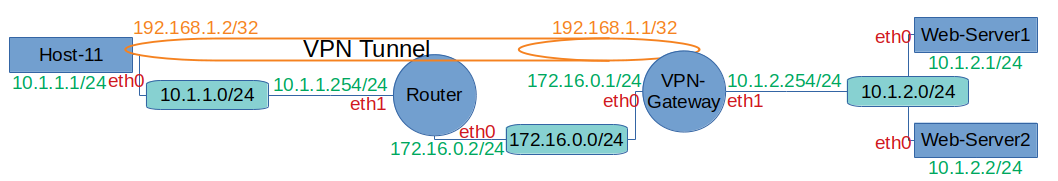
\includegraphics [width=0.8\textwidth]{labtainers-vpn2-lab-01.png}
\end{center}
\caption{Network topology for routing-basics lab}
\label{fig:topology}
\end{figure}

The network is composed of (find the main components of this network based on its topology):
\begin{itemize}
	\item
	\item
	\item
	\item
	\item
\end{itemize}

The OpenVPN application is pre-installed on the host and the server, and the OpenVPN configuration files already exist.

\section{Credentials}
\begin{itemize}
	\item \textbf{Host-11}:
	\begin{itemize}
		\item \textbf{Username:} user-11
		\item \textbf{Password:} user-11
	\end{itemize}
	\item \textbf{Web-Server1}:
	\begin{itemize}
		\item \textbf{Username:} web-admin
		\item \textbf{Password:} web-admin
	\end{itemize}
	\item \textbf{Web-Server2}:
	\begin{itemize}
		\item \textbf{Username:} web-admin
		\item \textbf{Password:} web-admin
	\end{itemize}
	\item \textbf{Router}:
	\begin{itemize}
		\item \textbf{Username:} admin
		\item \textbf{Password:} admin
	\end{itemize}
	\item \textbf{VPN-Gateway}:
	\begin{itemize}
		\item \textbf{Username:} admin
		\item \textbf{Password:} admin
	\end{itemize}
\end{itemize}

\section{Lab Tasks}

\subsection{Checking/Testing the Initial Configuration}\label{Checking/Testing the Initial Configuration}
Lets check what we can/can't do in this network.
\newline
\begin{itemize}
	\item On Host-11 (Check IP configuration and network interfaces)
	\begin{verbatim}
	    ip addr
	\end{verbatim}

	What is the result ? How many interfaces on the this machine ?

	\item On Router (Check IP configuration and network interfaces)
	\begin{verbatim}
	    ip addr
	\end{verbatim}

	What is the result ? How many interfaces on the this machine ?

	\item On VPN-Gateway (Check IP configuration and network interfaces)
	\begin{verbatim}
	    ip addr
	\end{verbatim}

	What is the result ? How many interfaces on the this machine ?

	\item On Host-11 (Ping Host-11 -$>$ Web-Server1)
	\begin{verbatim}
	    ping 10.1.2.1
	\end{verbatim}

	What is the result ? Why ? Is the server (private) network reachable from the host network ?

	\item On Host-11 (Ping Host-11 -$>$ Web-Server2)
	\begin{verbatim}
	    ping 10.1.2.2
	\end{verbatim}

	What is the result ? Why ? Is the server (private) network reachable from the host network ?

\end{itemize}

\subsection{Capturing the Traffic}
Lets use \textbf{tcpdump} which is a command line tool that can capture TCP/IP and other packets being transmitted or received over a network interface.
\newline
\newline
In the Router terminal, run the following command:
\begin{verbatim}
    sudo tcpdump -n -XX -i eth1
\end{verbatim}

Lets run tcpdump on Web-Server1 so we can monitor the traffic received on the server:
\begin{verbatim}
    sudo tcpdump -n -XX -i eth0
\end{verbatim}

\subsection{Configuring the VPN - VPN-Gateway Side}
\begin{itemize}
	\item Check VPN configuration

		\begin{verbatim}
				ls
		\end{verbatim}

		Notice that there are two files:

		\begin{itemize}
			\item gateway.conf: it contains the OpenVPN  configuration that will be used during establishing the VPN connection with the client.
				\begin{verbatim}
						cat gateway.conf
				\end{verbatim}

				The file content is as follows:
					\begin{itemize}
						\item The first line `dev tun` is the defining the type of the device/interface that will be created during the VPN establishment. In this case, we are using tunnel interface.
						\item The second line `ifconfig 192.168.1.1 192.168.1.2` defines the IP addresses of both end of tunnel.
						\item The third line `secret static.key` points to the file where the shared static key is stored.
						\item The fourth line `push "route 10.1.2.0 255.255.255.0"` advertises to the vpn-client that this network can be reached through the VPN-tunnel.
					\end{itemize}
			\item static.key: it contains the same secret key that exists on the client and will be used to establish the VPN connection with the client.
				\begin{verbatim}
						cat static.conf
				\end{verbatim}

		\end{itemize}

	\item Start the VPN connection on the VPN-Gateway.
		\begin{verbatim}
				sudo openvpn --config gateway.conf --daemon
		\end{verbatim}
\end{itemize}

\subsection{Configuring the VPN - Host/Client Side}
\begin{itemize}
	\item Check VPN configuration

		\begin{verbatim}
				ls
		\end{verbatim}

		Notice that there are two files:

		\begin{itemize}
			\item client.conf: it contains the OpenVPN  configuration that will be used during establishing the VPN connection with the VPN-Gateway.
				\begin{verbatim}
						cat client.conf
				\end{verbatim}

				The file content is as follows:
					\begin{itemize}
						\item The first line `remote 10.1.2.1` is the OpenVPN Gateway that it will connect to.
						\item The second line `dev tun` is the defining the type of the device/interface that will be created during the VPN establishment. In this case, we are using tunnel interface.
						\item The third line `ifconfig 192.168.1.1 192.168.1.2` defines the IP addresses of both end of tunnel.
						\item The fourth line `secret static.key` points to the file where the shared static key is stored.
						\item The fifth line `route 10.1.2.0 255.255.255.0 192.168.1.1 1` adds a new routing record to route thr traffic to this network through the tunnel interface. The `1` at the end of the line gives this route a higher priority than all other previous routes to the same network.
					\end{itemize}
			\item static.key: it contains the secret key that will be used to establish the VPN connection with the VPN-Gateway. This is a shared key, that means the VPN-Gateway should have the exact key in order to successfully establish the connection.
				\begin{verbatim}
						cat static.conf
				\end{verbatim}

		\end{itemize}

	\item Establishing the VPN connection.
		\begin{verbatim}
				sudo openvpn --config client.conf --daemon
		\end{verbatim}
\end{itemize}


\section{Testing the connectivity}
\begin{itemize}
	\item On Host-11 (Check IP configuration and network interfaces)
	\begin{verbatim}
	    ip addr
	\end{verbatim}

	What is the result ? How many interfaces on the this machine ?

	\item On VPN-Gateway (Check IP configuration and network interfaces)
	\begin{verbatim}
	    ip addr
	\end{verbatim}

	What is the result ? How many interfaces on the this machine ?

	\item On Host-11 (Ping Host-11 -$>$ Web-Server)
	\begin{verbatim}
	    ping 192.168.1.1
			wget 10.1.2.1
			ping 10.1.2.2
			wget 10.1.2.2
	\end{verbatim}

	What is the result ? Why do we used the private IP addresses not the tunnel ones ?

	\item Check the router terminal to see whether you still can find unencrypted text in the packets captured by the router.

	Check whether you can see the IP addresses (10.1.1.1, 10.1.2.1 or 10.1.2.2). Why can't you see any of them ?

	\item Check the server terminal and check which IP addresses you can see in the log. Can you see the IP address 10.1.1.1 ? Why ?

\end{itemize}

\section{Submission}
After finishing the lab, go to the terminal on your Linux system that was used to start the lab and type:
\begin{verbatim}
    stoplab sparta-vpn2
\end{verbatim}
When you stop the lab, the system will display a path to the zipped lab results on your Linux system.  Provide that file to
your instructor, e.g., via the Sakai site.

\end{document}
